\newcommand{\contentTablePage}{
    
    % шифр
    \begin{textblock*}{12cm}(8.5cm,25.8cm) 
        \centering 
        \chipher
    \end{textblock*}    

    % лист 3
    \begin{textblock*}{1.5cm}(17cm,27.3cm) 
        \centering 
        3
    \end{textblock*}   

    % листов общее кол-во
    \begin{textblock*}{2cm}(18.5cm,27.3cm) 
        \centering 
        \pageref{LastPage}
    \end{textblock*}  
    
    % уо бргту
    \begin{textblock*}{5cm}(15.5cm,28.3cm) 
        \centering 
        УО <<БрГТУ>>
    \end{textblock*} 

    % тема работы
    \begin{textblock*}{7cm}(8.5cm,26.8cm) 
        \centering 
        \theme
    \end{textblock*} 

    % мое фио
    \begin{textblock*}{2.3cm}(3.74cm,26.85cm) 
        \centering 
        {\fontsize{8pt}{9pt}\selectfont \student}
    \end{textblock*} 

    % фио преподавателя
    \begin{textblock*}{2.3cm}(3.74cm,27.35cm) 
        \centering 
        {\fontsize{9pt}{9pt}\selectfont \teacher}
    \end{textblock*} 


    % вставляем рамку
    % \AddToShipoutPictureBG{

    %     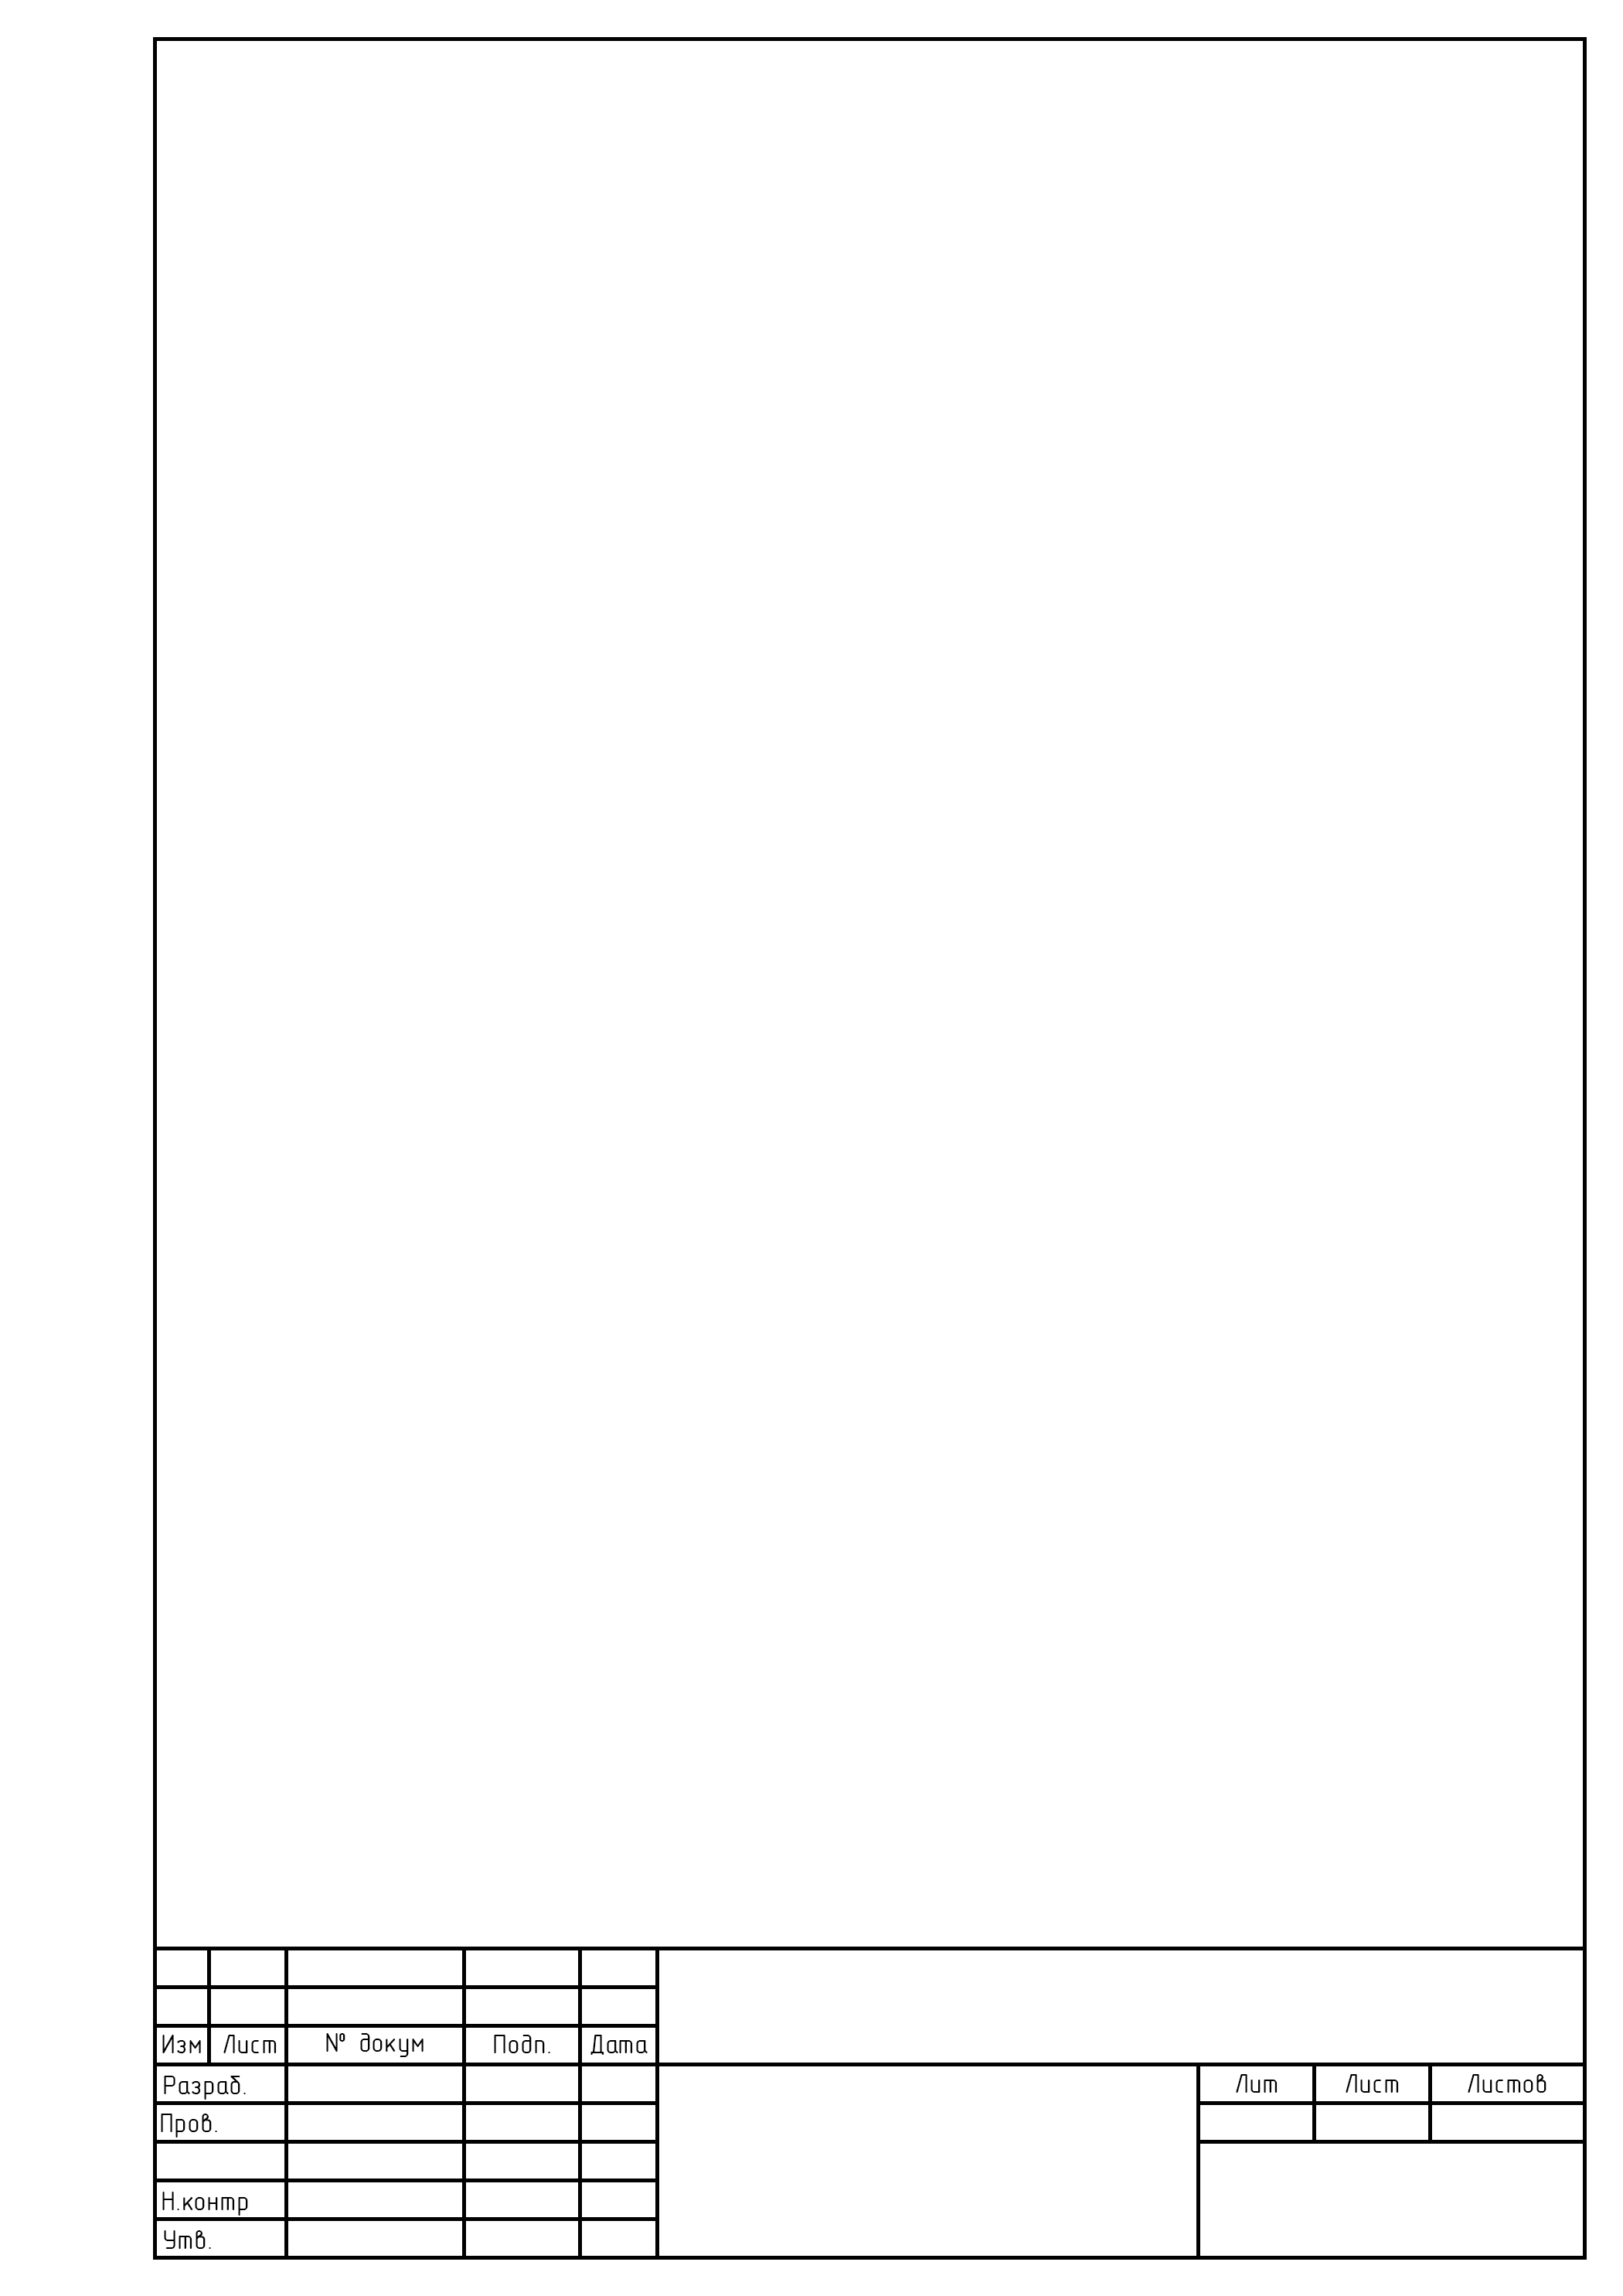
\includegraphics[width=\paperwidth,height=\paperheight]{border/border22.png}
    % }
    \backgroundsetup{
        scale=1,
        color=black,
        opacity=1,
        angle=0,
        position=current page.center,
        vshift=0cm, hshift=0cm,
        contents={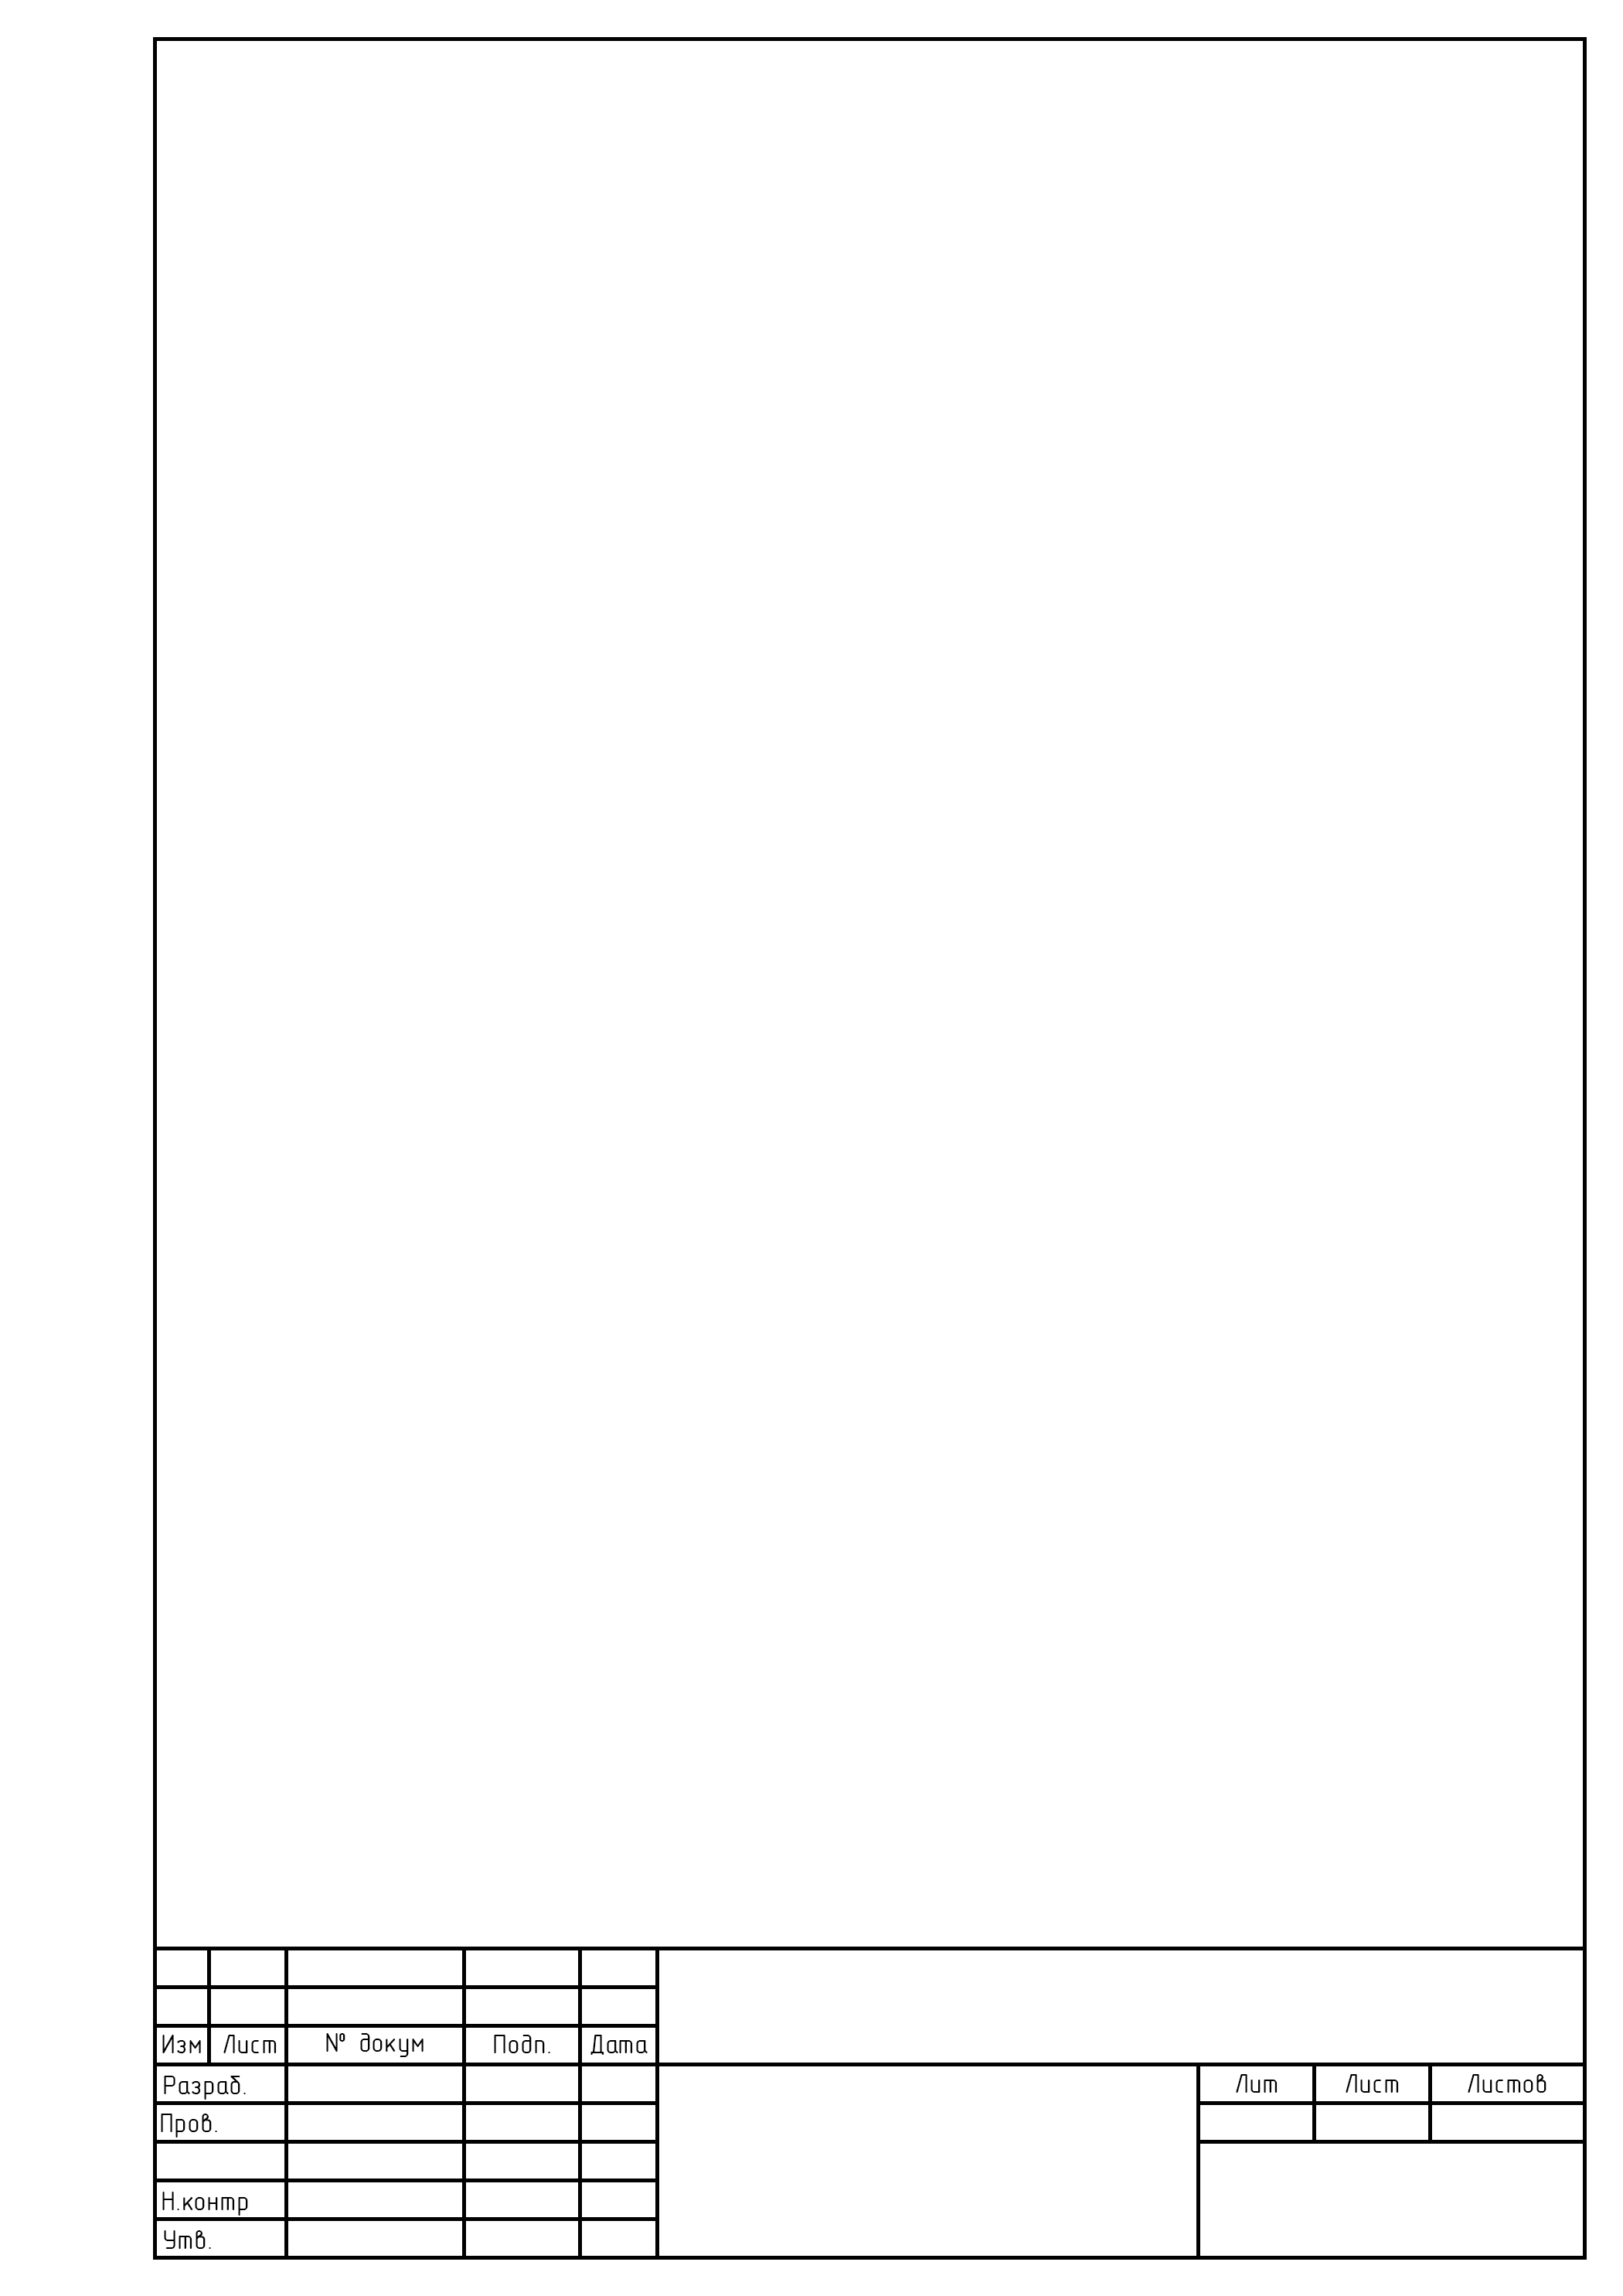
\includegraphics[width=\paperwidth,height=\paperheight]{border/border22.png}}
    }

    % номер для следующей страницы
    \AddToShipoutPicture{
                \begin{textblock*}{1cm}(19.5cm,28.6cm) 
                        \centering 
                        \number\numexpr\thepage+1\relax
                \end{textblock*}
        }
    
    % содержание
    \tableofcontents

    \newpage
    \ClearShipoutPicture

    \backgroundsetup{
                scale=3,
                color=black,
                opacity=0.1,
                angle=0,
                position=current page.south,
                vshift=5cm,
                hshift=0cm,
                contents={}
        }
}